\documentclass{beamer}
\usepackage{mathrsfs}  
\usepackage{xcolor}
\usepackage{setspace}
\usepackage{comment}
\usepackage[utf8]{inputenc}
\usepackage[T1]{fontenc}
\usepackage{centernot}
\usepackage{listings}
\usepackage{framed}





% config du thgeme metropolis
\usetheme[progressbar=frametitle,block=fill, titleformat=smallcaps,sectionpage=progressbar,]{metropolis}



\title{Rappels : Analyse Univariée et Bivariée}
\subtitle{}
\date{2021-2022}
\author{Paul Chapron \textsuperscript{1} \& Yann Ménéroux \textsuperscript{1}}
\institute{ \textsuperscript{1}IGN-ENSG-UGE}



%definition de la couleur du texte dans la balise \alert{}
\definecolor{vertIGN}{HTML}{96C31E} % vert IGN %vrai valeur #97BE0D
\setbeamercolor{alerted text}{fg=vertIGN}

\definecolor{grisIGN}{HTML}{22292F} % Gris IGN tiré vers le noir 
\setbeamercolor{background canvas}{bg=grisIGN}




% code pour placer le log ENSG dans le bandeau de titre 
\makeatletter
\setbeamertemplate{frametitle}{%
  \nointerlineskip%
  \begin{beamercolorbox}[%
      wd=\paperwidth,%
      sep=0pt,%
      leftskip=\metropolis@frametitle@padding,%
      rightskip=\metropolis@frametitle@padding,%
    ]{frametitle}%
  \metropolis@frametitlestrut@start%
  \insertframetitle%
  \nolinebreak%
  \metropolis@frametitlestrut@end%
  \hfill
  \raisebox{-0.6ex}{\includegraphics[height=4ex,keepaspectratio]{img/logoENSG_small.jpg}}
  \end{beamercolorbox}%
}
\makeatother




% logo ENSG première page 
\titlegraphic{\vspace{4cm}\flushright\includegraphics[width=2cm,height=2cm]{img/logoENSG_big.png}} 



\begin{document}
\metroset{background=dark} % change background theme according to manual
\maketitle	

\section{Introduction} 

\begin{frame}{Dans les cours précédents ... }


Notions pour manipuler les \alert{variables aléatoires}, et estimer certains descripteurs

\begin{itemize}
\item co-variance
\item intervalle de confiance 
\item bootstrap
\item \dots
\end{itemize}

\end{frame}


\begin{frame}{Motivation}


L'analyse \alert{univariée} permet de \alert{décrire la forme}  et de \alert{quantifier} les caractéristiques de  la \alert{répartition des valeurs} d'une variable.



\begin{itemize}
	\item Notion de distribution 
	\item Visualisation ( Histogramme, densité, boxplots, \dots)
	\item Moments, Quantiles, CV 
\end{itemize}
\end{frame}






\section{Analyse Univariée}



\begin{frame}{Histogramme}

 \begin{block}{Histogramme d'une variable}
Représentation graphique des \alert{effectifs} associés à des \alert{classes de valeurs} d'une variable numérique 
\end{block}

Le nombre de classes peut varier ! 


\begin{figure}[!htb]
   \begin{minipage}{0.5\textwidth}
     \centering
     \includegraphics[width=.9\linewidth]{img/histogramme1.png}
     
   \end{minipage}\hfill
   \begin{minipage}{0.5\textwidth}
     \centering
     \includegraphics[width=.9\linewidth]{img/histogramme2.png}
     
   \end{minipage}
\end{figure}




\end{frame}


\begin{frame}{Distribution}

\begin{tiny}
  Synonymes: distribution empirique, distribution des fréquences, distribution statistique
\end{tiny}

\alert{Tableau} ou \alert{graphique} qui associe les (classes de) valeurs à leur \alert{fréquence d'apparition}


$\approx$ « Histogramme des fréquences en continu»


\begin{figure}
  \centering
     \includegraphics[width=.7\linewidth]{img/densité.png}
\end{figure}
\end{frame}

\begin{frame}{Distribution}





La distribution peut être définie comme une \alert{fonction} qui donne la probabilité qu’un individu $x$ pris au hasard  ait la valeur $V_x$ pour la variable $V$ : 

$$distribution(V) \equiv P(V=V_x),\forall V_x \in \Omega_V$$ 

Avec $\Omega_V$  l’ensemble des valeurs que peut prendre V : l’univers de V

Lorsque la variable prend des valeurs réelles, on parle de \alert{densité de probabilité}, c’est pourquoi on retrouve ce terme “density” sur les axes des ordonnées dans les graphiques de distribution.


\end{frame}

\begin{frame}{Distribution et histogramme}

\begin{figure}
  \centering
     \includegraphics[width=.7\linewidth]{img/histo_dens.png}
\end{figure}

\begin{small}
\begin{spacing}{0.75}
\alert{N.B.} En toute rigueur, représenter une courbe de distribution de probabilité par dessus un histogramme est impropre : il faudrait deux graphiques distincts, ou au moins deux axes des ordonnées: un pour l’histogramme, représentant un effectif, l’autre pour la distribution , représentant une probabilité 
\end{spacing}
\end{small}

\end{frame}





\begin{frame}{Distribution et lois}

Parfois , les distributions empiriques ressemblent à celles de lois de probabilités connues. 

$\rightarrow$ on peut alors  \alert{modéliser}  la  variable par une variable aléatoire de loi fixée

$\rightarrow$ les paramètres de cette loi doivent être déterminés (ajustement).


\end{frame}


\begin{frame}{Décrire une distribution}


La forme d'une distribution donne beaucoup d'informations  : 

\begin{small}
\begin{itemize}
  \setlength\itemsep{-0.0em}
  \begin{spacing}{0.7}
 \item \alert{"pics"} : valeurs les plus représentées dans la population 
 \item présence de \alert{valeurs extrêmes} : la courbe de la distribution est tirée à gauche ou à droite du graphique
 \item \alert{symétrie} : les individus se répartissent équitablement de part et d'autre du pic  
 \item \alert{aplatissement} : la population est plus ou moins resserrée, ou  autour de certaines valeurs 
 \item \dots
 \end{spacing}
\end{itemize}
\end{small}

\begin{figure}
  \centering
     \includegraphics[width=.65\linewidth]{img/densité.png}
\end{figure}



\end{frame}


\section{Décrire une distribution : mesures de \alert{tendance centrale}}

\begin{frame}{Tendance Centrale}


La tendance centrale est \alert{une} valeur qui \alert{résume} une série de valeurs (quantitative)

\vspace{1cm}


\begin{itemize}
  \item Moyenne
  \item Médiane 
  \item Mode
\end{itemize}


\end{frame}


\begin{frame}{Moyenne}


$$ \bar{x} = \frac{1}{n}\sum_{i=0}^{n} x_i$$


\begin{spacing}{0.9}
\begin{small}
Avantage  : chaque valeur compte  \\
Inconvénients : \\ 
\begin{itemize}
  \item sensibilité aux valeurs extrêmes 
  \item pas de signification sur les valeurs discrètes (e.g. 2.5 enfants par foyer)
\end{itemize}

Pour y remédier (parfois): \\
$\rightarrow$ exclure les outliers\\
$\rightarrow$ utiliser un autre estimateur (médiane)\\
$\rightarrow$ étudier la distribution des valeurs (e.g. cas bimodal) et opérer une classification
\end{small}
\end{spacing}

\end{frame}



\begin{frame}{Moyenne géométrique}

$$ \bar{x}_{geom} = \sqrt[n]{\prod _{i=0}^{n} x_i}$$  


Moins sensible que la moyenne classique aux valeurs extrêmes.

\end{frame}



\begin{frame}{Mode}


Le \alert{mode} d’une variable est la valeur la plus \alert{fréquente} ( d’effectif maximum) d’une variable.
\begin{spacing}{0.9}
\begin{small}
Avantages  : 
\begin{itemize}
  \item peu sensible aux valeurs extrêmes 
  \item interprétation  simple : cas le plus fréquent
\end{itemize}  
Inconvénient :  la valeur du mode ne dépend pas de toutes les observations, la modification d'une valeur n'entraîne pas la modification du mode (ce qui explique sa robustesse aux valeurs extrêmes)

\end{small}
\end{spacing}

\end{frame}



\begin{frame}{Calcul du mode}
Si la variable est quantitative et continue : 
\begin{itemize}
  \item découper l’étendue de la variable ($max -min$) en intervalle égaux
  \item compter les effectifs de chaque intervalle
  \item le mode est la moyenne des valeurs des bornes de l'intervalle de plus grand effectif.
\end{itemize}

\begin{tiny}
(C’est exactement ce que fait un histogramme graphiquement !)
\end{tiny}

\end{frame}



\begin{frame}{Modes}

Par définition, le mode est unique, mais on peut appeler modes les valeurs des autres pics d’une distribution.\\

 On parle de distribution \alert{bi-modale} ou \alert{tri-modale} lorsqu’une distribution présente deux ou trois pics. 

 Les \alert{valeurs modales} d’une distribution sont les valeurs correspondant à ces pics. 



\begin{figure}
  \centering
     \includegraphics[width=.7\linewidth]{img/trimodale.png}
\end{figure}

\end{frame}


\begin{frame}{Médiane}

La \alert{médiane} est la valeur qui sépare une population en \alert{deux} classes d'égal effectif.\\

C'est la valeur la plus proche de toutes les autres.


\begin{spacing}{0.9}
\begin{small}
Avantages  : 
\begin{itemize}
\item Souvent plus pertinente que la moyenne
\item les valeurs extrêmes ne modifient pas sa valeur
\item interprétation  facile: un individu sur deux a une valeur inférieure (respectivement supérieure) à la médiane.
\end{itemize}
\end{small}
\end{spacing}


Inconvénient : Comme le mode , la médiane ne dépend pas de toutes les observations 

\begin{tiny}
\begin{spacing}{0.9}
\alert{N.B.} la robustesse de la médiane est bien utile dans le cas de distribution particulièrement asymétriques, où la moyenne est dégradée par les valeurs extrêmes, à droite (valeurs très élevées) ou à gauche (valeurs très faibles).
\end{spacing}
\end{tiny}

\end{frame}




\begin{frame}{Moyenne et médiane}

Que peut on dire d'une population dont la médiane est inférieure à la moyenne ? 


Exemple : revenus mensuels en équivalent temps plein en France en 2016.

Revenu mensuel net moyen 2 238 €\\
Revenu mensuel net médian 1 789 € 

\vspace{2cm}
\begin{tiny}
source \url{https://www.insee.fr/fr/statistiques/4277680?sommaire=4318291}
\end{tiny}


\end{frame}



\begin{frame}{Moyenne et médiane}

Un salaire mensuel net équivalent temps plein de 2000€ est-il un bon salaire ? 

\begin{itemize}
  \item 2000€  <  moyenne  :  on peut le considérer comme trop bas pour être «bon»
  \item 2000€ > médiane  :  supérieur à (au moins) la moitié des salaires du pays, on peut le considérer comme un «bon» salaire.
\end{itemize}

\begin{small}
Double interprétation  \& «instinctivement» on imagine une dispersion symmétrique, où la moyenne est proche de la médiane 
\end{small}


\end{frame}




\section{Décrire une distribution : mesures de \alert{dispersion}}

\begin{frame}{Dispersion}


La  \alert{dispersion} décrit  la tendance des valeurs d'une variable à se disperser plus ou moins largement autour des valeurs des tendances centrales.

\end{frame}


\begin{frame}{Variance et écart type}

La \alert{variance} est la somme des écarts carrés à la moyenne rapporté à l'effectif

$$ var_X= \frac{1}{n}\sum_{i=1}^{n}(x_i -\bar{x})^2$$

Avec :
\begin{itemize}
  \item $X$ une variable
  \item $x_i$ les valeurs de la variables
  \item $\bar{x}$ la moyenne de $X$ 
  \item $n$ l'effectif
\end{itemize}


\end{frame}


\begin{frame}{Variance et écart type}


L'\alert{écart type} est la racine carrée de la variance


$$\sigma_X = \sqrt{var_X}$$ 



Variance et écart-type sont sensibles aux valeurs extrêmes et toujours positifs.\\





\begin{tiny}
\begin{spacing}{0.8}
Si $var_X = 0$ ou $\sigma_X = 0$ , alors $X$ est \alert{constante}.\\
Un écart-type faible indique que les valeurs sont réparties de façon \alert{homogène} autour de la moyenne.
\end{spacing}
\end{tiny}



\end{frame}


\begin{frame}{Quantiles}
 

La \alert{médiane} sépare une population en \alert{deux} classes d'égal effectif 

Les \alert{quantiles}  séparent une population en \alert{$n$} classes d'égal effectif.
\end{frame}


\begin{frame}{Quartiles}




Les \alert{quartiles} d'une population selon une variable $X$ sont trois valeurs, $Q_1,Q_2,Q_3$ qui séparent la population en \alert{quatre} classes d'égal effectif.

\begin{itemize}
  \item 25\% des valeurs de $X$ sont strictement inférieures à $Q_1$
  \item 50\% des valeurs de $X$ sont strictement inférieures à $Q_2$ (médiane)
  \item 75\% des valeurs de $X$ sont strictement inférieures à $Q_3$
\end{itemize}
\end{frame}


\begin{frame}{Déciles}



Les déciles sont les \alert{9} quantiles $Q_1,Q_2,\dots,Q_9$ qui séparent une population  \alert{10} classes d'égal effectif.

\end{frame}


\begin{frame}{Écarts inter-quartiles et inter-déciles}


\alert{Écart inter-quartile}: $Q_3-Q_1$ , capture 50\% des valeurs de la population les plus proches de la médiane

\vspace{1cm}


\alert{Écart inter-décile}: $Q_9-Q_1$ , capture 80\% des valeurs de la population les plus proches de la médiane

\end{frame}


\begin{frame}{Quantiles}




\begin{columns}[T,onlytextwidth]
\column{0.48\textwidth}
\begin{block}{Avantages}

Peu sensibles aux distributions aplaties et aux valeurs extrêmes

L'écart inter-quantile est plus robuste que l'écart-type
\end{block}
\column{0.4\textwidth}
\metroset{block=fill}

\begin{block}{Inconvénients}

Parfois délicat pour les variables quantitatives discrètes

Les écarts inter-quantiles négligent l'influence des valeurs extrêmes sur la distribution
\end{block}


\end{columns}







\end{frame}

\begin{frame}{Les boîtes à moustaches (boxplots)}


\vspace{1cm}
Représentation courante de la dispersion d'une variable à l'aide de \alert{quartiles}



\begin{columns}[T,onlytextwidth]
\column{0.48\textwidth}

\centering
\includegraphics[width=\linewidth]{img/boxplot.png}

\column{0.5\textwidth}
\metroset{block=fill}
\begin{scriptsize}
\begin{itemize}
\item La \alert{marque centrale} de la boîte est la \alert{médiane}
\item Les \alert{bords} de la boîte sont les \alert{quartiles $Q_1$ et $Q_3$}
\item Les moustaches vont jusqu'à la plus grande (resp. la plus petite ) valeur inférieure (resp. supérieure)  à \alert{1.5 fois l’écart interquartile} 
\item Les valeurs qui dépassent les moustaches sont affichées sous formes de points
\end{itemize}
\end{scriptsize}
\end{columns}

\end{frame}



\begin{frame}{Le coefficient de variation}

Le \alert{coefficient} de variation ($CV$) est une autre mesure de dispersion.

C'est le ratio entre l'écart-type $\sigma_x$ et la moyenne $\bar{x}$ d'une variable quantitative $X$.

$$ CV(X)=\frac{\sigma_x}{\bar{x}}$$

Plus il est important , plus la dispersion est grande.

Plus il est proche de 0, plus les données sont homogènes.


Inconvénients similaires à ceux de  $\bar{x}$ et $\sigma_x$ : sensibilité aux valeurs extrêmes.


\end{frame}

\begin{frame}{Comparaison de dispersion de deux distributions}



Exemple : deux communes  versent des aides aux entreprises locales, qu'on suppose distribuées suivant une loi normale. 

Commune A :  moyenne = 390 euros, $\sigma$ = 30 euros 

Commune B :  moyenne = 152 euros, $\sigma$ = 8 euros

\vspace{1cm}

Pour quelle commune les aides sont les plus homogènes?



\end{frame}





\section{Décrire une distribution : \alert{asymétrie} et \alert{aplatissement}} 



\begin{frame}{Asymétrie (ou \alert{skewness})}




\centering
\includegraphics[width=\linewidth]{img/asymetrie.png}



\end{frame}


\begin{frame}{Coefficients d'asymétrie de Pearson}


Deux moyens simples d'estimer l'asymétrie 

$$ C_1 = \frac{\bar{x} - mode(X)}{\sigma_x}$$

$$ C_2 = \frac{3(\bar{x} - mediane(X))}{\sigma_x}$$

\begin{itemize}
  \item coefficient \alert{nul} :  la distribution est \alert{symétrique}
  \item coefficient \alert{négatif} : la distribution est \alert{déformée à gauche} de la médiane (sur-représentation de valeurs faibles, à gauche)
  \item coefficient \alert{positif} :  la distribution est \alert{déformée à droite} de la médiane (sur-représentation de valeurs fortes, à droite)
\end{itemize}


\end{frame}


\begin{frame}{ Coefficient d'asymétrie de Fischer}


Ce coefficient est le moment  d'ordre 3  de la variable $X$ ( de moyenne $\mu$ et d'écart-type $\sigma$) \alert{centrée réduite}

$$skewness'=\mathbb{E}\bigg[\bigg(\frac{X-\mu}{\sigma}\bigg)^3\bigg]=\frac{\sum_{i=0}^{n} (x_i - \bar{x})^3}{n\sigma^3}$$


Interprétation similaire aux coefficients de Pearson  




\end{frame}




\begin{frame}{Aplatissement  (ou \alert{Kurtosis})}


\begin{center}
\includegraphics[width=\linewidth]{img/aplatissement.png}
\end{center}

Courbe piquée: Peu de variation, distribution relativement homogène, beaucoup de valeurs égales ou proches de la moyenne.

Courbe aplatie: Variations importantes, distribution relativement hétérogène, beaucoup de valeurs s’éloignent de la moyenne.

\end{frame}



\begin{frame}{Coefficient de Kurtosis}




$$ K=\frac{\sum_{i=1}^{n}(x_i -\bar{x})^4}{n\sigma^4}$$

Si la distribution est normale, $K= 3$

Si $K>3$, la distribution est \alert{plus aplatie} 

Si $K<3$, la distribution est \alert{moins aplatie} 

On normalise parfois en considérant $K'=K-3$ (quantifie l'excès d'aplatissement)


\end{frame}


\section{Analyse Bivariée}

\begin{frame}{Analyse bi-variée}


Étude de  la relation entre \alert{deux} variables : 

\begin{itemize}
  \item quantitatives : \alert{corrélation, régression linéaire}
  \item qualitatives : test d'indépendance du \alert{«Chi deux» / $\chi^2$}
\end{itemize}

\vspace{2cm}

\begin{scriptsize}
\begin{spacing}{0.75}
Pour le lien entre une variable quantitative et une variable qualitative, on fera simplement un graphique.
\end{spacing}
\end{scriptsize}


\end{frame}







\begin{frame}{Corrélation $\neq$ Causalité }




 Une liaison, même très forte, entre deux variables, n’indique pas la causalité. 

\begin{figure}
  \centering
     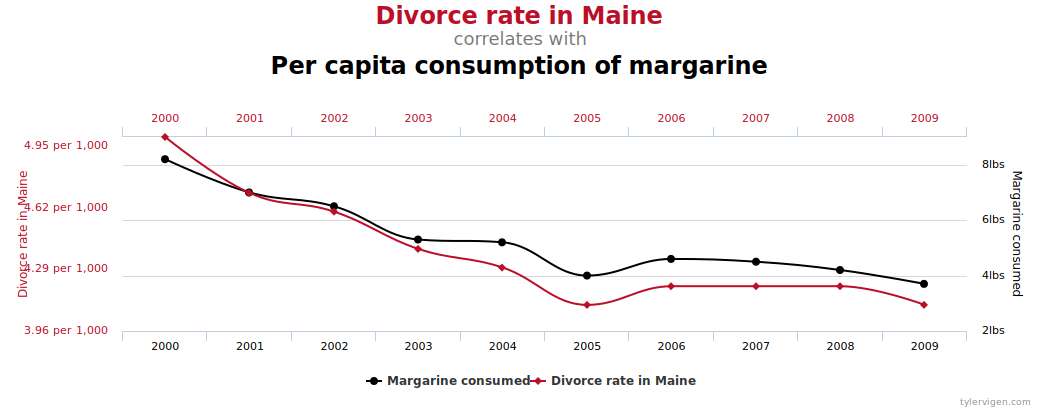
\includegraphics[width=.9\linewidth]{img/spurious.png}
\end{figure}

Erreur très courante , très tentante. 

\end{frame}


\begin{frame} {Analyse bivariée avec des données spatiales}


\begin{block}{\alert{Données «spatiales»}}

Individus restreints spatialement (sélection spatiale)


Variables “géographique” (e.g. lieu de résidence) renseignées pour les individus

Prise en compte des distances $\rightarrow$ modèle(s) gravitaire(s) (hors programme)
\end{block}

\vspace{1cm}

\begin{block}{Données localisées (hors programme pour nous)}

    Auto-corrélation spatiale (Moran’s I, Geary Index)

    Geographically Weighted Regression (GWR) $\approx$ régression linéaire avec prise en compte de la distance entre individus

    Variogrammes 
\end{block}

\end{frame}



\section{Corrélation}

\begin{frame}{Avant toute chose}

\alert{Toujours} afficher les données, avant de faire quoi que ce soit.



\begin{figure}
  \centering
     \includegraphics[width=\linewidth]{img/correlation_examples2.png}
\end{figure}



\end{frame}




\begin{frame}{Corrélation de Pearson}


La \alert{corrélation} indique l’\alert{intensité} du lien \alert {linéaire} entre deux variables quantitatives.





$$cor(x,y)\in[-1;1]$$



\begin{itemize}
  \item $cor(x,y)\approx0$ : pas de relation (\alert{linéaire}) entre les deux variables

  \item $cor(x,y)<0$  : les deux variables ont des sens de variations opposés
  \item $cor(x,y)>0$  : les deux variables varient conjointement 

  \item $cor(x,y)= \pm 1$ : variables parfaitement linéairement (anti-)corrélées, i.e. fonction affine l'une de l'autre. 
\end{itemize}

\end{frame}


\begin{frame}{Formule du coefficient de corrélation de Pearson }


$$r= \frac{cov(x,y)}{\sigma_x\sigma_y}=\frac{E\big[(x-E(x))(y-E(y))  \big]}{\sigma_x\sigma_y}$$ 

Avec : 

\begin{itemize}
  \item $r$ (parfois $\rho$) le coefficient de corrélation
  \item $x$ et $y$ deux variables quantitatives
  \item $E(x)$ l'espérance d'une variable $x$
  \item $\sigma_x$ l'écart-type  d'une variable $x$
  \item $cov(x,y)$ la covariance  de deux variables  $x$ et $y$
\end{itemize}


\end{frame}





\begin{frame}{Corrélation et indépendance }
\begin{small}
Deux variables indépendantes ont un coefficient de corrélation nul :
$$ x \perp\!\!\!\!\perp y \implies  cor(x,y)=0  $$
MAIS une corrélation nulle n'\alert{implique pas} l'indépendance des variables ! 
$$cor(x,y)=0 \centernot \implies x \perp\!\!\!\!\perp y $$
\end{small}
D'autres liaisons sont possibles : 


\begin{figure}
\includegraphics[width=.32\linewidth]{img/sinus.png}
\includegraphics[width=.33\linewidth]{img/flou.png}
\includegraphics[width=.32\linewidth]{img/quadratic.png}
\end{figure}



\end{frame}


\begin{frame}[fragile]{Corrélation avec R }


Fonction  $\texttt{cor(x,y)}$  pour obtenir la valeur du coefficient,

Fonction $\texttt{cor.test(x,y)}$ pour obtenir  la \alert{p-value} et \alert{l'intervalle de confiance}. 


Résultat :

\begin{scriptsize}
\begin{spacing}{0.75}
\begin{lstlisting}[language=R,basicstyle=\footnotesize\ttfamily, commentstyle=\ttfamily]
## 
##  Pearson's product-moment correlation
## 
## data:  iris$Petal.Length and iris$Petal.Width
## t = 43.387, df = 148, p-value < 2.2e-16
## alternative hypothesis: true correlation
## is not equal to 0
## 95 percent confidence interval:
##  0.9490525 0.9729853
## sample estimates:
##       cor 
## 0.9628654
\end{lstlisting}
\end{spacing}
\end{scriptsize}








\begin{scriptsize}
\begin{spacing}{0.75}
R donne le coefficient de Pearson par défaut, l’argument  $\texttt{method}$ de la fonction cor() permet de spécifier deux autres coefficients : Kendall et Spearman.
\end{spacing}
\end{scriptsize}

\end{frame}


\begin{frame}[fragile]{Matrice de Corrélation}

Fonction $\texttt{cor()}$  appliquée à plusieurs variables de type $\texttt{numeric}$

e.g. $\texttt{cor(iris[,1:4])}$


Résultat: 

\begin{tiny}
\begin{spacing}{0.75}
\begin{lstlisting}[language=R,basicstyle=\scriptsize\ttfamily, commentstyle=\ttfamily]
##              Sepal.Length Sepal.Width Petal.Length Petal.Width
## Sepal.Length    1.0000000  -0.1175698    0.8717538   0.8179411
## Sepal.Width    -0.1175698   1.0000000   -0.4284401  -0.3661259
## Petal.Length    0.8717538  -0.4284401    1.0000000   0.9628654
## Petal.Width     0.8179411  -0.3661259    0.9628654   1.0000000
\end{lstlisting}
\end{spacing}
\end{tiny}




Présentation des corrélations entre les variables quantitatives d’un tableau, pour tous les couples de variables.

La matrice de corrélation est symétrique, et sa diagonale est constituée de 1.

\end{frame}



\begin{frame}[fragile]{Sensibilité aux outliers}



\begin{tiny}
\begin{spacing}{0.75}
\begin{lstlisting}[language=R,basicstyle=\scriptsize\ttfamily, commentstyle=\ttfamily]
X <-  c(3,2,3,4,1,2,3,4,5,2,3,4,3)
Y <-  c(1,2,2,2,3,3,3,3,3,4,4,4,5)
plot(X, Y, xlim = c(0,16), ylim= c(0,16))
\end{lstlisting}
\end{spacing}
\end{tiny}




\begin{figure}
\includegraphics[width=.9\linewidth]{img/outlier1.png}
\end{figure}



\begin{tiny}
\begin{spacing}{0.75}
\begin{lstlisting}[language=R,basicstyle=\scriptsize\ttfamily, commentstyle=\ttfamily]
>cor.test(X,Y)$estimate
## cor 
##   0
\end{lstlisting}
\end{spacing}
\end{tiny}

\end{frame}




\begin{frame}[fragile]{Sensibilité aux outliers}



\begin{tiny}
\begin{spacing}{0.75}
\begin{lstlisting}[language=R,basicstyle=\scriptsize\ttfamily, commentstyle=\ttfamily]
X <-  c(3,2,3,4,1,2,3,4,5,2,3,4,3,15)
Y <-  c(1,2,2,2,3,3,3,3,3,4,4,4,5,15)
plot(X, Y, xlim = c(0,16), ylim= c(0,16))
\end{lstlisting}
\end{spacing}
\end{tiny}




\begin{figure}
\includegraphics[width=.9\linewidth]{img/outlier2.png}
\end{figure}



\begin{tiny}
\begin{spacing}{0.75}
\begin{lstlisting}[language=R,basicstyle=\scriptsize\ttfamily, commentstyle=\ttfamily]
>cor.test(X,Y)$estimate
## cor 
##   0.9052224
\end{lstlisting}
\end{spacing}
\end{tiny}

\end{frame}



\begin{frame}{Outliers}


\alert{Outlier} : observation “anormale”, par ses valeurs extrêmes, comparées aux autres.

La corrélation (et la régression linéaire)) sont très sensibles aux outliers.

$\rightarrow$ s’interroger sur la nécessité de nettoyer/filtrer les données et les conséquences

$\rightarrow$ ne pas faire d’épuration brutale et aveugle

\end{frame}



\begin{frame}{Coefficient de corrélation de Spearman}



Quand les deux variables semblent corrélées , de façon \alert{monotone} mais \alert{non linéaire},

$\rightarrow$ utiliser le coefficient de \alert{Spearman}, basé sur le \alert{rang} des individus.


$$\rho_S= \frac{cov(rg_x, rg_y)}{\sigma_{rg_x}\sigma_{rg_y}}$$


Avec :
\begin{itemize}
  \item $rg_x$ le rang des individus selon la variable $x$  (en cas d'ex-aequo on prend le rang moyen)
  \item $cov()$ la fonction de covariance
  \item $\sigma_{rg_x}$ l'écart-type du rang $rg_x$
\end{itemize}



\end{frame}


\section{Régression linéaire}

\begin{frame}{Régression linéaire}


\alert{Toujours} afficher les données, avant de faire quoi que ce soit.


\alert{Si} le nuage de points semble «suffisament» linéaire , on peut tenter de décrire la relation statistique linéaire en proposant un \alert{modèle}

$$\hat{y} = \alpha x + \beta$$



\end{frame}





\begin{comment}




\begin{frame}{Animation}
  \begin{itemize}[<+- | alert@+>]
    \item \alert<4>{This is\only<4>{ really} important}
    \item Now this
    \item And now this
  \end{itemize}
\end{frame}



\begin{frame}[standout]
Mono message sur une diapo
\end{frame}
\end{comment}

\end{document}